\documentclass[12pt,compress,ngerman,utf8,t]{beamer}
\usepackage[ngerman]{babel}
\usepackage[protrusion=true,expansion=true]{microtype}
\usepackage{booktabs}

\DeclareSymbolFont{extraup}{U}{zavm}{m}{n}
\DeclareMathSymbol{\varheart}{\mathalpha}{extraup}{86}
\DeclareMathSymbol{\vardiamond}{\mathalpha}{extraup}{87}

\title{Die Vielfalt freier Lizenzen}
\author[Linux User Group Augsburg e.V.]{Ingo Blechschmidt}
\date{Linux User Group Augsburg \\ 1. Juni 2016}

\usetheme{Warsaw}

\useinnertheme{rectangles}

\usecolortheme{seahorse}
\definecolor{mypurple}{RGB}{150,0,255}
\setbeamercolor{structure}{fg=mypurple}

\usefonttheme{serif}
\usepackage{bookman}

\setbeamertemplate{navigation symbols}{}
\setbeamertemplate{headline}{}
\setbeamertemplate{frametitle}[default][colsep=-2bp,rounded=false,shadow=false,center]

\renewcommand*\insertshorttitle{Die Vielfalt freier Lizenzen
  \hfill \insertframenumber\,/\,\inserttotalframenumber {\quad}}

\newcommand{\hil}[1]{{\usebeamercolor[fg]{item}{\textbf{#1}}}}

\begin{document}

\frame{\titlepage}

\begin{frame}\frametitle{Die Kathedrale und der Basar}
  \centering
  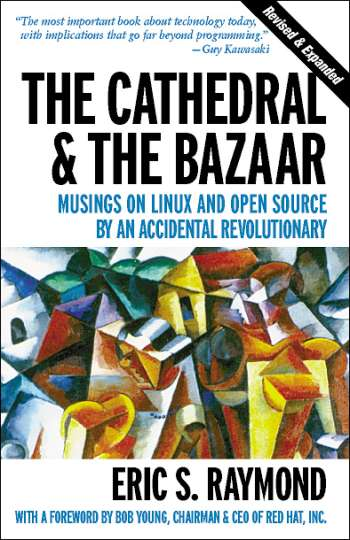
\includegraphics[height=0.85\textheight]{images/cathedral-bazaar}
  \par
\end{frame}

\begin{frame}\frametitle{Die vier wesentlichen Freiheiten}
  \begin{center}
    
\includegraphics[scale=0.3]{images/gnu}
  \end{center}

  Software ist \hil{frei}, wenn man \ldots
  \medskip

  \begin{enumerate}
    \addtocounter{enumi}{-1}
    \item sie zu jedem Zweck ausführen,
    \item sie untersuchen und verändern,
    \item sie verbreiten und
    \item Verbesserungen verbreiten darf.
  \end{enumerate}
\end{frame}

\begin{frame}[c]\frametitle{Virales Copyleft}
  \centering
  
\includegraphics[height=3.5cm]{images/richard-stallman}
  \qquad
  
\includegraphics[height=3.5cm]{images/copyleft}
  \par
\end{frame}

\begin{frame}[c]\frametitle{Wo sieht man die Lizenzen?}
  \Huge
  \centering
  \textsl{Demo}
  \par
\end{frame}

\begin{frame}\frametitle{Beispiele für Lizenzen}
  \small\centering
  \begin{tabular}{lllll}
    \toprule
    Lizenz & Linking & Verteilung & Veränderung & Copyleft \\\midrule
    GPL & verboten\footnote{nur in GPL-kompatible Software} & erlaubt & erlaubt & ja \\
    LGPL & erlaubt\footnote{mit Einschränkungen} & erlaubt & erlaubt & nein \\
    MIT & erlaubt & erlaubt & erlaubt & nein \\
    BSD & erlaubt & erlaubt & erlaubt & nein \\
    CC0 & erlaubt & erlaubt & erlaubt & nein \\
    \bottomrule
  \end{tabular}\par
\end{frame}
% XXX: Patenttrollschutz?
% XXX: nc-Lizenzen

\end{document}
